\documentclass[../main.tex]{subfiles}

\begin{document}

\chapter{Benchmark Comparison}

We now have a data-driven methodology for deriving learned sector universes (addressing RG-1), and have developed a objetive criteria-driven ranking methodology to compare the learned sector universes against each other, addressing RG-2. The final step is to evaluate our objectively-identified risk-adjusted return optimal learned sector universe (see Section~\ref{optimal_sector_universe:risk_adj_return_optimal}) against the benchmark classification. Thus, this section addresses the third and final research goal, RG-3 (see Section~\ref{research_goals:specific_research_goals}).

\begin{table}[h!]
    \centering
    \begin{tabular}{| c | c |}
        \hline
        &  \\
        RG-3 & Evaluate our risk-adjusted return optimal sector universe against the benchmark. \\
        & \\
        \hline
    \end{tabular}
\end{table}

\section{Comparison Overview}

To preserve the impartial basis for comparison developed and maintained throughout this report, we isolated sector assigments for our benchmark sector universe, the \textit{GICS S\&P 500 Classification}. Unfortunately, as mentioned previously, we were only able to isolate transverse sector assignments for the year 2019, and were unable to access historical sector assignments, thus making a truly longitudinal comparison of our learned sector to the benchmark impossible.

To mitigate this issue, we compared the latest learned sector as implied by our clustering algorithm to the benchmark classification. To maintain the consistency of our analysis, we utilized reIndexer (see Section~\ref{candidate_universe_ranking:reindexer}) to model SETFs of the benchmark, and to perform a backtest using the same configuration as was used for the candidate learned sector ranking (see Section~\ref{candidate_universe_ranking:backtest_config}). Similarly, we utilized the same performance metrics as were used to compare the candidate learned sector universes (see Section~\ref{candidate_universe_ranking:eval_metrics}) to compare the risk-adjusted return optimal learned sector universe to the benchmark.

\section{Performance Metric Comparison}

Figure~\ref{fig:benchmark_comparison:performance_metrics} contains four panels, (a) through (d), with each displaying one of the four performance metrics outlined in Section~\ref{candidate_universe_ranking:eval_metrics}. To best decompose the results of the comparison with the \textit{GICS S\&P 500 Classification} benchmark, we will analyze each of the performance metric comparisons in turn.

\subsection{Cumulative Turnover Comparison}

Panels (a) and (b) in Figure~\ref{fig:benchmark_comparison:performance_metrics} plot the cumulative turnover of SETF restructuring, and portfolio rebalancing, respectively. Recall from the previous section that for these turnover metrics, lower is better. As the red line represents the benchmark, it is apparent that the risk-adjusted return optimal learned sector did not outperform the benchmark with respect to both the SETF restructuring turnover, and the portfolio rebalancing turnover.

This phenomenon may be explained through analysis of the Sankey Diagram of the risk-adjusted return learned sector universe in Figure~\ref{fig:optimal_sector_universe:max_sharpe}. It indicates a significant proliferation of component assets in 2 large sectors, with a large number of smaller sectors. Due to the fact that larger sectors have a higher notional value, and thus imply higher turnover when bought or sold, it is not surprising that the portfolio rebalancing turnover is higher for the risk-adjusted return optimal learned sector univese, compared to the more uniformly distributed benchmark universe.

Additionally, the larger individual sectors \textit{Alpha} and \textit{Golf} would also imply a higher rate of turnover during SETF restructuring. As a higher number of assets implies a more volatile total value, the extremely large sectors unique to the risk-adjusted return optimal learned sector universe would command a higher level of turnover during SETF restructuring, when compared to the more modestly sized sectors of the benchmark universe.

% See: https://tex.stackexchange.com/questions/238923/refer-to-a-table-as-figure
\begin{table}[!h]
    \centering
    % \fbox{
    \begin{tabular}{|c|c|}
        \hline
        & \\
        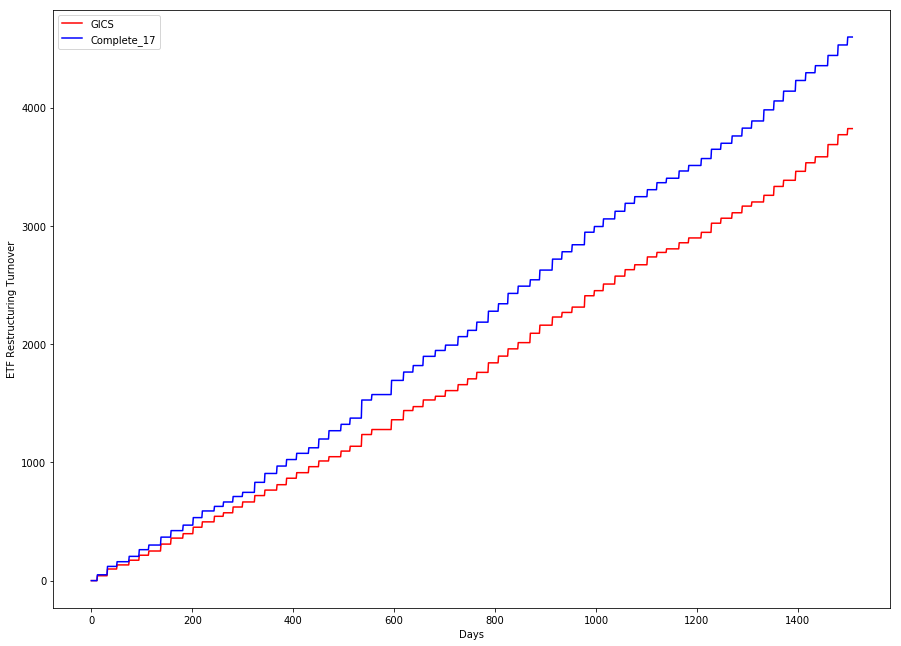
\includegraphics[width=.48\linewidth]{images/etf_restrut_compare.png} &
        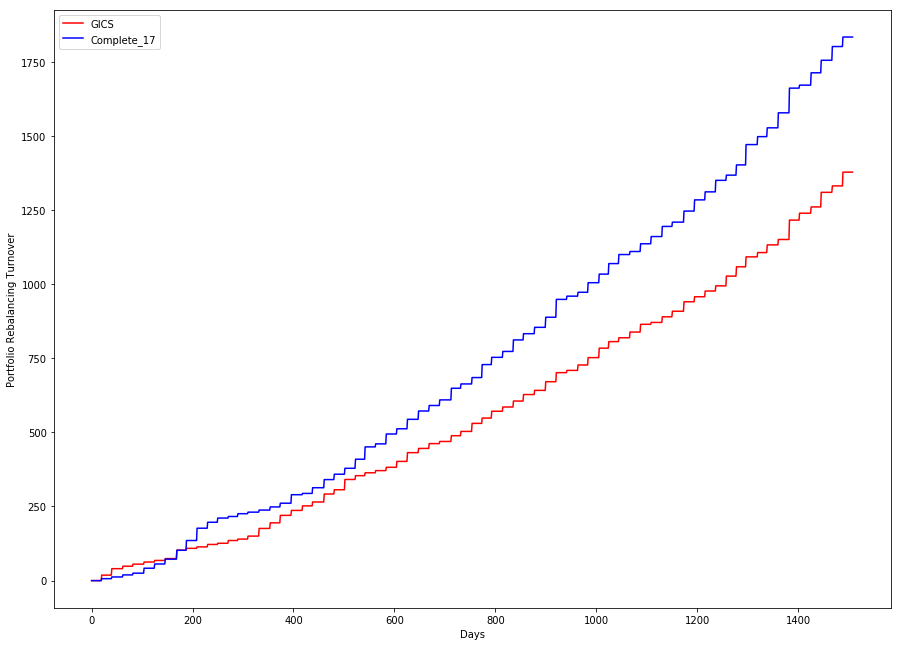
\includegraphics[width=.48\linewidth]{images/port_rebal_compare.png} \\
        \textit{(a) SETF Restructuring Turnover} & \textit{(b) Portfolio Rebalancing Turnover} \\
        & \\
        \hline
        & \\
        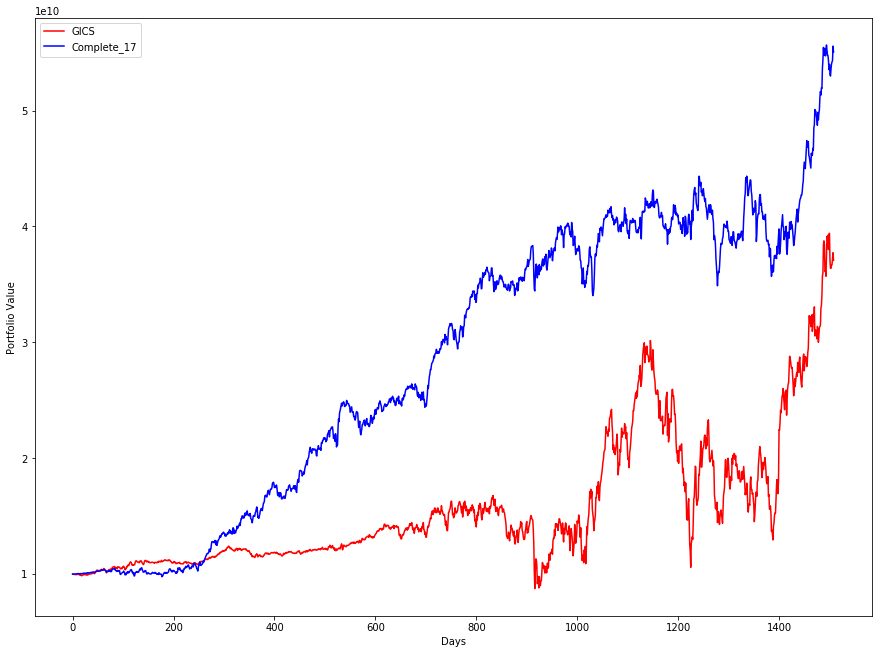
\includegraphics[width=.48\linewidth]{images/value_compare.png} &
        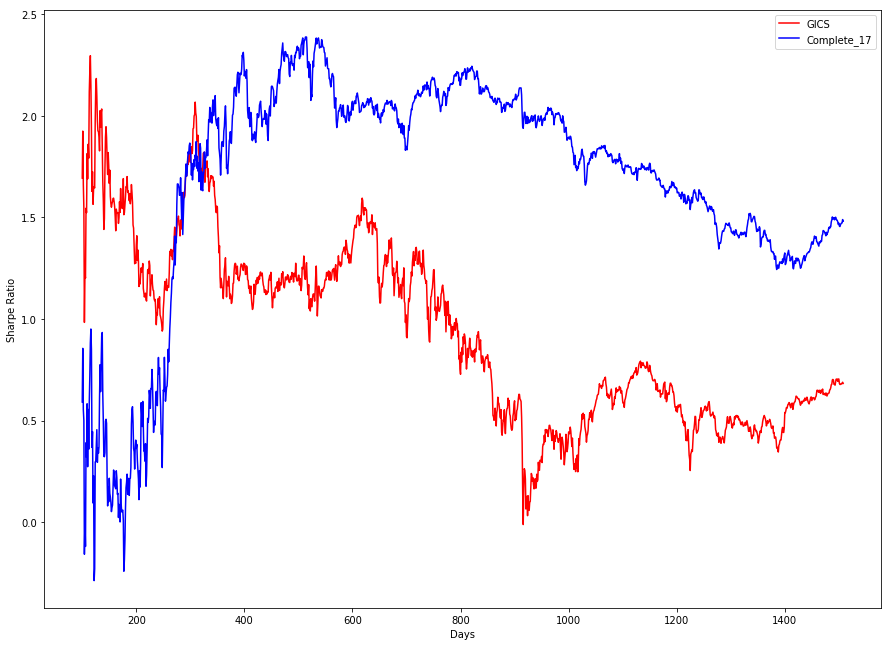
\includegraphics[width=.48\linewidth]{images/sharpe_compare.png} \\
        \textit{(c) Absolute Portfolio Value} & \textit{(d) Risk-adjusted Return} \\
        & \\
        \hline
    \end{tabular}
    % }
    \captionof{figure}{A comparison of sector universe performance metrics, with the \textcolor{red}{benchmark universe in red}, and the \textcolor{blue}{risk-adjusted return optimal learned sector universe in blue}.}
    \label{fig:benchmark_comparison:performance_metrics}
\end{table}


\subsection{Absolute Portfolio Value Comparison}

Panel (c) in Figure~\ref{fig:benchmark_comparison:performance_metrics} is a comparison of the absolute portfolio value of both the risk-adjusted return optimal learned sector universe, and the benchmark universe. As indicated by the graph, the learned sector universe provides a significantly higher value at the terminus of the backtest, beating out the benchmark by nearly \$15,000,000,000 on a starting capital base of \$10,000,000,000 each, which translates to an outperformance of nearly 150\%.

The progression of the portfolio over time for both the learned sectors universe and the benchmark universe indicate that the portfolio returns of the two sector universes are lightly correlated. This is to be expected, as the underlying base of investable assets is identical (by design) between the two sector universes. However, there does appear to be significantly less historical volatility in the returns of the learned sector universe portfolio compared to the benchmark portfolio.

This is particularly evident in the 750 - 1250 day interval in panel (c). This period shows that the portfolio value of the benchmark increased rapidly, at a significantly greater rate than its learned sector universe counterpart. However, at approximately the 1150 day mark, the benchmark suffers a extremely severe drop, losing nearly all of its gains of the preceeding period.

Interestingly, the learned sector universe portfolio does not appear to fluctuate in value significantly (relative to the benchmark) during this period. This observation, coupled with the commensurate final rally in both sector universe portfolios near the end of the backtesting period suggests that the diversification profile of the learned sectors portfolio is \textit{significantly} superior to that of the benchmark, resulting in not only a higher terminal portfolio value, but also significantly less volatility in reaching that value.

\subsection{Risk-Adjusted Return Comparison}

Figure~\ref{fig:benchmark_comparison:performance_metrics} (d) is a comparison of the rolling risk-adjusted return (i.e. Sharpe Ratio) of the benchmark sector universe and the risk-adjusted return optimal learned sector universe. Given the results of the analysis of the absolute portfolio value comparison above, the outperformance of the learned sector universe relative to the benchmark universe is not a surprising result.

Continuing on the same line of analysis as the previous section, the Sharpe ratio of the benchmark sector universe performs extremely poorly during the interval of 750 - 1250 days discussed above. The negative effect of the increased volatility, despite a rally in the underlying portfolio is better reflected in the Sharpe ratio plot compared to the portfolio value plot of panel (c). In fact, the Sharpe ratio graph in panel (d) indicates that it was nearly more beneficial to own and hold the risk-free asset than the benchmark sector universe portfolio at approximately the 900 day mark, as the rolling Sharpe ratio fo the portfolio briefly approaches 0. Despite rallying significantly during the interval, the Sharpe ratio of the benchmark sector universe never recovers, and does not approach the significantly higher value of the learned sector univese portfolio.

Additionally, despite rallying toward the end of the backtest, the Sharpe ratio plots indicate that the trend of the rolling risk-adjusted return for both sector universes was negative, with a much more smooth slope on the learned sector universe portfolio line. This indicates a lower \textit{vol of vol} for the learned sector universe compared to the benchmark universe, which is further indication that the learned sector algorithm provides significantly better diversification benefits compared to the benchmark sector universe.

% Yuzhen's stuff
% In this chapter we make comparison between our optimal sector universe of maximum Sharpe Ratio and benchmark sector universe. We compare each of the performance metric of both sector universes and demonstrate which sector universe has better risk-adjusted return.  

% \section{Comparison Analysis}

% Our benchmark sector universe is GICS S\&P 500 sectors universe. We do the backtesting of benchmark sector universe and calculate the same index we talk about in above chapters, which are cumulative ETF restructuring turnover, cumulative portfolio rebalancing turnover, portfolio return and portfolio Sharpe Ratio  respectively. The graphs of comparison between benckmark sector universe and our optimal sector unverse are:

% All red curves represent performances of benchmark sector universe and all blue curves represent performance optimal sector universe with Complete Linkage,16 Sectors. The graphs show that for cummulative turnovers,benchmark sector universe perform better than our optimal universe. One possible reason is the structure of our optimal sector. We will explore the relationship of sector structure and turnover in future work. 

% Back to the topic, we highlight the comparison of Sharpe Ratio since it reflect the risk-adjusted return. From the graph, it is clear that the Sharpe Ratio of our optimal sector universe is higher than that of benchmark sector universe for most of the time during backtesting period. This indicates that our sector universe from machine-learning algorithm has hagher risk-adjusted return rhan benchmark. 


\section{Qualitative Comparison}

In this section, we attempt to conduct a more qualitatively-driven comparison and contrast of the risk-adjusted return optimal learned sector universe against the benchmark sector universe. Given the drastic difference in performance between the benchmark sector universe portfolio and the optimal learned sector unviverse portfolio, we believe that there is significant insight to be had by analyzing the composition of each of the sectors in the universe.

Analyzing each of the learned sectors in turn (from Figure~\ref{fig:optimal_sector_universe:max_sharpe} and Figure~\ref{fig:benchmark_comparison:ls_optimal_assets}), it is clear that beyond the large sectors \textit{Alpha} and \textit{Golf}, a large majority of the remaining sectors are extremely small with respect to their numbers of component assets. Despite this however, the two large (major) sectors - as well as a selection of the smaller (i.e. minor) sectors - have an extremely high dispersion rate relative to the benchmark. That is, there doesn't seem to be a high level of congruence between the old and new sector assignments. This lack of agreement between the benchmark and learned sector universes is particularly apparent in the apparent lack of any direct transitional sector mappings in Figure~\ref{fig:benchmark_comparison:ls_optimal_assets}.

Both major learned sectors \textit{Alpha} and \textit{Golf} comprise a large number of assets as their components. Particularly, it can be observed that learned sector \textit{Alpha} contains a majority of the benchmark \textit{Financials} sector, and the benchmark \textit{Utilities} sector. Given that these sector assignments are derived from fundamentals data, this is a particularly interesting result, as both \textit{Financials} and \textit{Utilities} have become extremely risk-averse businesses over the last decade; \textit{Financials} due to the Great Recession of 2008, and \textit{Utilities} due to extensive capital damange incurred by the increased severity and number of Natural Disasters. This grouping indicates that the capital structure of these businesses are also becoming increasingly similar.

\begin{figure}[!h]
    \centering
    \fbox{
    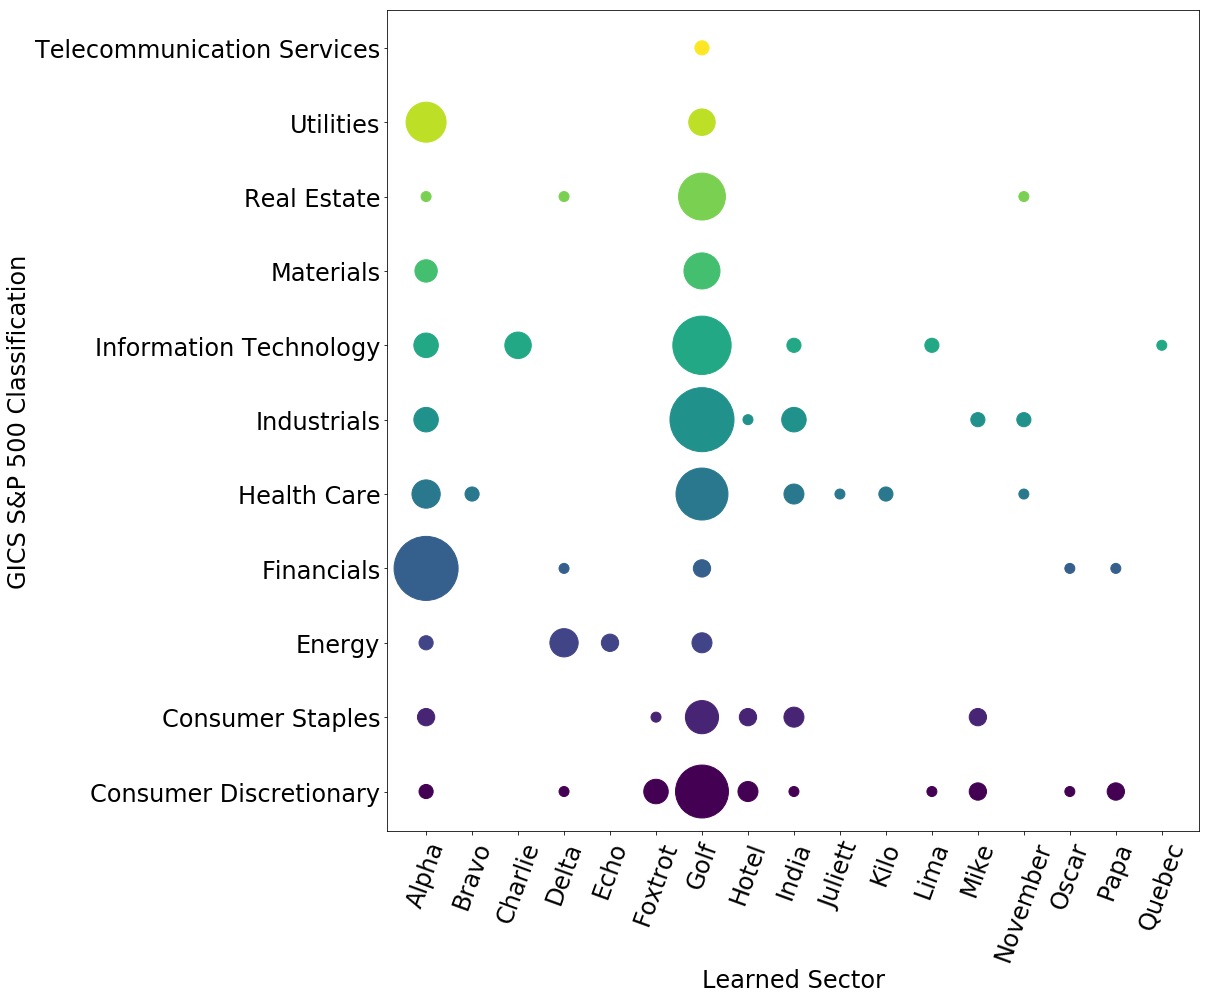
\includegraphics[width=.7\linewidth]{images/complete_17_benchmark_diff.png}
    }
    \caption{Sector assignment transitions between the benchmark sector classification universe and the risk-adjusted return optimal learned sector universe.}
    \label{fig:benchmark_comparison:ls_optimal_assets}
\end{figure}

Considering learned sector \textit{Golf}, it seems to be a mini-index within the oringal sector universe. From a component count perspective, it ingests a large amount of the benchmark \textit{Consumer Discretionary} and \textit{Consumer Staples} industries, as well as large swaths of industries that form the backbone of the US Economy as a whole; namely, the \textit{Information Techonology}, \textit{Industrials}, and \textit{Real Estate} sectors.

Appendix~\ref{appendix:portfolio_weights} contains stacked bar charts representing the level of investment in each of the sector SETFs for both the benchmark sector universe (see Figure~\ref{fig:appendix_weights:benchmark}), and the risk-adjusted return optimal learned sector universe (see Figure~\ref{fig:appendix_weights:sharpe_optimal}). Analyzing these graphs, in conjunction with the transition profile of sector assignments between the benchmark and optimal learned sector universe, it is clear that the learned sector \textit{Golf} was not a strong performer. The benefit of containing a large cross-section of companies from myriad traditional sectors, combined with their poor performance during the years of 2014 and 2015 appears to be a key factor in the outperformance of the benchmark sector universe.

\end{document}